\chapter{2014年财务预算}
\section{2014年度财务预算编制说明}

\renewcommand{\labelenumi}{\indent (\chinese{enumi})}
\begin{enumerate}
\setlength{\itemindent}{1.3em} %标签缩进量
% \setlength{\parsep}{0ex} %段落间距
 \setlength{\topsep}{1ex} %列表到上下文的垂直距离
 \setlength{\itemsep}{0.5ex} %条目间距

\item 编制依据
  \begin{enumerate}[1、]
\item 根据川渝工业有限责任公司2013年卷烟产销计划,预计全年生产滤棒164亿支、销售164亿支;根据川渝中烟工业公司2013 年实际嘴棒结算价、单位平均实际销售成本、职工薪酬和制造费用按上年口径测算,预计销售收入64282万元,利税总额必保6\%,6100万元,力争8\%,6200万元。

\item 丝束等原辅料采购成本按川渝中烟工业有限责任公司核定现行进口、国产丝束价测算。
\end{enumerate}

\item 费用说明

严格控制可控费用支出,但职工薪酬、折旧等刚性费用会有所增加,预计2014年度管理费用3044万元,较上年增加57万元;经营费用817万元,较上年增加202万元;重点费用开支控制在上年实际内(详见~\ref{section:Budge}~节的预算方案)。
\end{enumerate}
%%%%%%%%%%%%%%%%%%%%%%%%%%%%%%%%%%%%%%%%%%%%%%%%%%%%%%%
\section{2014年度财务预算方案}\label{section:Budge}
\subsection{主要财务指标预算编制情况}
\begin{table}[!htpb]
 \centering
  \begin{threeparttable}[b]
    \renewcommand{\arraystretch}{1.3}
 \centering  \caption{2014年主要财务指标预算编制情况}
\rowcolors{2}{darkblue!20}{white}  %% start_row:odd_color:even_color
       \begin{tabular}
   {@{}>{\sf
   }p{0.25\textwidth}<{\centering}p{0.15\textwidth}<{\centering}p{0.15\textwidth}<{\centering}p{0.15\textwidth}<{\centering}p{0.15\textwidth}<{\centering}@{}}
    \spacecell{} & \spacecell{} & \spacecell{} & \spacecell{} &  \spacecell{{单位:万元}}\\
  \toprule[1pt]

   \sf 预算项目&\sf	2014年预算	&\sf 2013年实际	&\sf 增减额&	\sf 增减率\\
\midrule
销售收入&64282 &62091 &2191 &4\%\\
销售成本&    55,989 &53463 &2526 &5\%\\
三项费用(不含薪酬)&1819.86&1508.41&311 &21\%\\
销售费用&537.56&398.17&139 &35\%\\
管理费用&1289.82&1116.15&174 &16\%\\
财务费用&-7.52&-5.91&-2&27\%\\
制造费用(不含薪酬)&3112.98&2696.46&417 &15\%\\
利润总额&4143&4869&-726&-15\%\\
税利总额&6200&5740&460 &8\%\\

\bottomrule[1pt]
 \end{tabular}
 \end{threeparttable}
 \end{table}


\subsection{重点预算项目编制}
具体见表~\ref{table:Bz}。
\begin{table}[!htpb]
\centering
  \begin{threeparttable}[b]
    \renewcommand{\arraystretch}{1.3}
 \centering  \caption{2014年行业重点预算项目编制情况}\label{table:Bz}
\rowcolors{2}{darkblue!20}{white}  %% start_row:odd_color:even_color
       \begin{tabular}
   {@{}>{\sf
   }p{0.25\textwidth}<{\centering}p{0.15\textwidth}<{\centering}p{0.15\textwidth}<{\centering}p{0.1\textwidth}<{\centering}p{0.3\textwidth}<{\centering}@{}}
    \spacecell{} & \spacecell{} & \spacecell{} & \spacecell{} &  \spacecell{{单位:万元}}\\
  \toprule[1pt]
  \sf 五项重点费用&	\sf 2014年预算&	\sf 2013年实际&	\sf 增减额&	\sf 备注\\
\midrule
业务招待费&115&110.71 &4.29 &控制在上年实际以内\\
宣传促销费&80&2.24 &77.76 &上年执行延后\\
会议费&15.02&0.18 &14.84 &上年未执行\\
涉外费&55&26.49 &28.51 &计划涉外培训\\
福利费&350&317.02&32.98 &根据工资总额14\%\\
\bottomrule[1pt]
 \end{tabular}
 \end{threeparttable}
 \end{table}



\subsection{投资预算}
以川渝公司下达的年度投资计划执行。

%%%%%%%%%%%%%%%%%%%%%%%%%%%%%%%%%%%%%%%%%%%%%%%%%%%%%%%%%%%%%%%%%%%%%%%%%%%%%%%%%%%%%%
\section{2014年薪酬分配预案}


根据川渝烟工人[2013]~572号《关于下达2013年度工资总额的通知》,2013年我公司工资总额为2287.5万元。按川渝公司要求,2014 年工资总额预算按2013 年实发工资总额编制。因工资总额预期不增加,加之国家对相关行业职工工资管控力度加强,2014年工资总额控制难度增加。
按现工资分配体系,本着先紧后松,留有余地、尽可能均衡发放,严控年度工资总额的原则,2014年度薪酬计划使用总额为2287.5万元,具体如下:

%%%%%%%%%%%%%%%%%%%%%%%===Fig6-1===%%%%%%%%%%%%%%%%%%
\begin{figure}[htbp]
  \centering
 % \includegraphics[scale=1.0,bb=123 686 460 585,clip]{Fig2-1.pdf}
  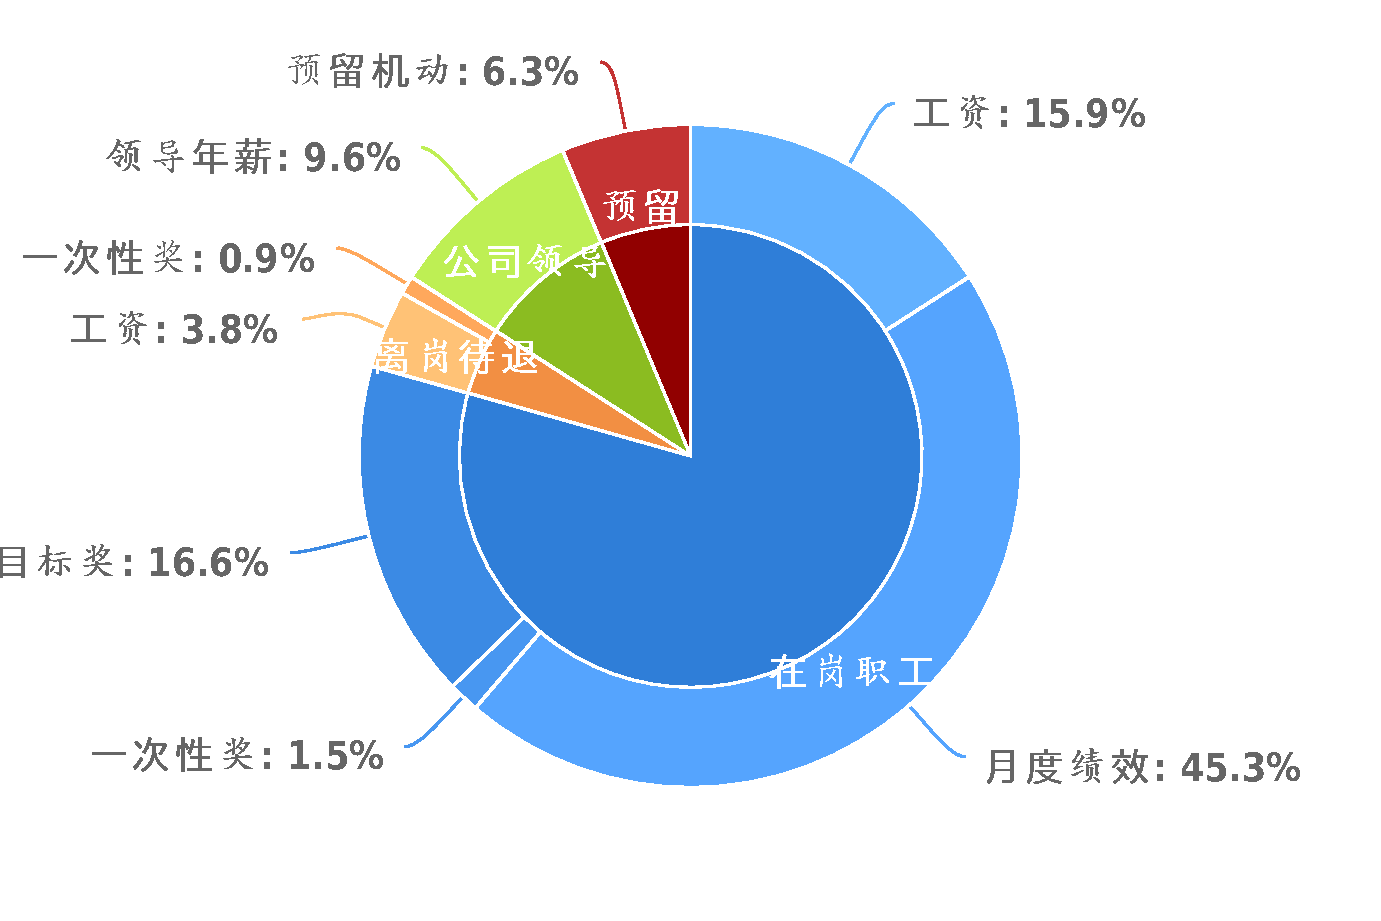
\includegraphics[width=0.8\textwidth]{fig6_1.pdf}
  \caption{2014年薪酬分配预案}
  \label{figure2}
\end{figure}
%%%%%%%%%%%%%%%%%%%%%%%===Fig6-1===%%%%%%%%%%%%%%%%%%

一、在岗职工部分,预计总使用计划额度为18166000元,其中工资计划使用额度为3646000元,月度绩效计划使用额度为10373000元,目标奖计划使用额度为3800000元,一次性奖计划使用额度347000元。

二、离岗待退职工部分,预计总使用计划额度为1078188元,其中工资计划使用额度为860988元,一次性奖计划使用额度为217200元。


三、公司领导部分,预计年薪使用额度为2188000元。

四、预留机动额度为1442812元。




